\section{\textit{Statistical Learning}}

Per poter analizzare un \textit{learning algorithm} c'è bisogno di definire un 
modello matematico di come gli esempi $(x,y)$ siano generati. Nel contesto della
\textit{statistical learning} si assumerà che ogni esempio sia ottenuto attraverso
un'estrazione indipendente da una distribuzione di probabilità fissata su
$\X \times \Y$. Si scriverà $(X,Y)$ per sottolineare come 
\textbf{le due componenti di un esempio siano due variabili aleatorie}.

Assumere che ogni esempio $(x,y)$ sia la realizzazione di un'estrazione casuale 
\textbf{indipendente} da un'unica distribuzione $\D$, implica che ogni 
\textit{dataset} (come \textit{test} e \textit{training set}) sia un campione
statistico. L'indipendenza dei dati è in realtà violata in alcuni domini pratici.
Nonostante ciò, l'assunzione di indipendenza nei dati è estremamente utile dal
punto di vista della tracciabilità analitica del problema e funziona
sorpendentemente bene nella pratica.

\subsection{Definizioni}
Nel contesto della \textit{statistical learning} un problema è specificato da una
coppia $(\D,\ell)$, dove $\D$ è la distribuzione e $\ell$ la \textit{loss function}.

\subsubsection{Rischio statistico \texorpdfstring{$\ell_{\D}$}{lD}}
Le prestazioni di un predittore $h:\X \rightarrow \Y$ rispetto a $(\D,\ell)$ è 
valutata dal \textbf{rischio statistico}:
$$ \ell_{\D}(h) = \E[\ell(Y,h(X))] $$
che indica il valore atteso della \textit{loss function} su un esempio casuale 
$(X,Y)$ estratto da $\D$.

\subsubsection{Predittore ottimo di Bayes \texorpdfstring{$f^*$}{f*}}
Data $\D$, il miglior predittore possibile $f^*:\X \rightarrow \Y$ è detto 
\textbf{predittore ottimo di Bayes}:
$$ f^*(x) = \argmin_{\hat{y} \in \Y} \E[\ell(Y,\hat{y})\ | \ X=x] $$

\subsubsection{Rischio condizionato}
L'argomento di $\argmin$ di $f^*$, ovvero $\E[\ell(Y,\hat{y})\ | \ X=x]$, è detto
\textbf{rischio condizionato}. Il \textit{Bayes optimal predictor} quindi, è la 
predizione che minimizza il rischio condizionato. Un altro modo per scrivere il
rischio condizionato di un predittore $f$ è:
$$ \E[\ell(Y,\hat{y})\ | \ X=x] = \E[\ell(Y,f(X))\ | \ X=x] $$

\subsubsection{Rischio di Bayes \texorpdfstring{$\ell_{\D}(f^*)$}{lDF*}}
Essendo $f^*$ il miglior predittore possibile per $\D$ è ragionevole pensare che
esso abbia il rischio statistico migliore, ed è così; si ha infatti che il rischio 
$\ell_{\D}(f^*)$, detto \textbf{rischio di Bayes}, è il minore tra tutti i
predittori:
$$ \forall h \in \F \quad \ell_{\D}(f^*) \leq \ell_{\D}(h) $$
Tipicamente il rischio di Bayes è maggiore di zero vista la casualità delle
etichette.

\subsection{
    \texorpdfstring{$f^*$}{f*} e \texorpdfstring{$\ell_\D$}{lD*} nelle varie
    \textit{loss function}
}
Si valuteranno ora i predittori ottimi di Bayes per le varie \textit{loss function}.
\subsubsection{\textit{Quadratic loss}}

Sia $\ell(y,\hat{y}) = (y-\hat{y})^2 \ \text{con } \Y = \RN $.

Si analizzi il predittore ottimo di Bayes:
\begin{align}
    f^*(x) &= \argmin_{\hat{y}\in\RN} \E[(Y-\hat{y})^2 \ | \ X=x]  \notag\\
           &= \argmin_{\hat{y}\in\RN} \E[Y^2+\hat{y}^2-2\hat{y}Y\ | \ X=x]\notag\\[.6em]
        \multispan2{Per le varie proprietà del valore atteso si ha:\hfil} \notag\\[.6em]
           &= \argmin_{\hat{y}\in\RN}
            \left({\E[Y^2\ | \ X=x]}+\E[\hat{y}^2\ | \ X=x]-\E[2\hat{y}Y\ | \ X=x]\right)
            \notag\\[.6em]
           &= \argmin_{\hat{y}\in\RN}
           \left({\color{red}\E[Y^2\ | \ X=x]}+\E[\hat{y}^2\ | \ X=x]-2\hat{y}\E[Y\ | \ X=x]\right)
           \notag\\[.6em]
        \multispan2{Siccome $\argmin$ varia su $\hat{y}$, tutti {\color{red}i fattori che non ne dipendono}\hfil
        } \notag\\
        \multispan2{non incidono sul risultato; possono quindi essere tolti:\hfil
        } \notag\\[.6em]
        &= \argmin_{\hat{y}\in\RN}
           \left(\E[{\color{blue}\hat{y}}^2\ | \ X=x]-2\hat{y}\E[Y\ | \ X=x]\right)
           \notag\\[.6em]
        \multispan2{Non essendo ${\color{blue}\hat{y}}$ una variabile aleatoria:\hfil
           } \notag\\[.6em]
        &= \argmin_{\hat{y}\in\RN}
            \left({\color{blue}\hat{y}^2}-2\hat{y}\E[Y\ | \ X=x]\right) \notag
\end{align}
L'argomento di $\argmin$ è una funzione del tipo:
\begin{equation}
    F(\hat{y}) = \hat{y}^2 -2\hat{y}q \tag*{$q=\E[Y\ | \ X=x]$}
\end{equation}
Obiettivo di argmin è trovare il valore di $\hat{y}$ che minimizza $F$. Facendo 
un semplice studio di funzione si può trovare che $F$ è minimizzata quando:
$$
\begin{aligned}
    \multispan2{$F'(\hat{y}) = 2\hat{y}-2q$} \\
    \multispan2{Cerco il minimo:\hfill}\\
    F'(\hat{y}) &= 0\\
    2\hat{y}-2q &= 0\\
    \hat{y}     &=q\\
\end{aligned} \qquad \Rightarrow \qquad \hat{y}=\E[Y\ | \ X=x]
$$

\textbf{Si può quindi dire che}:
$$ f^*(x) = \E[Y\ | \ X=x]  = \E[Y\ | \ X]$$

Sostituendo il risultato appena mostrato nella formula del rischio condizionato
si ha:
$$ \begin{aligned}
    \ & \E[\ell(Y,\hat{y})\ | \ X=x] \\ 
    = \ &\E[(Y-f^*(X))^2\ | \ X=x] \\
    = \ &\E[(Y-\E[Y \ | \ X ])^2\ | \ X=x] \\
    = \ & \var[Y \ | \ X]
\end{aligned} $$

\textbf{Il rischio di Bayes sarà quindi}:
$$ \ell_\D(f^*) = \E[\var[Y \ | \ X]] \neq \var[Y] $$

Da notare che il valore atteso della varianza dato $X$ sia diverso dalla varianza;
per la legge della varianza totale si ha infatti che:
$$ \var[Y]-\E[\var[Y \ | \ X]] = \var[\E[Y \ | \ X]] $$

\subsubsection{\textit{Zero-one loss}}
Si guarderà ora la classificazione binaria dove $\Y = \{-1,1\}$.

Si definiscano due funzioni:
\begin{align}
\eta(x) = \Prob(Y=1 \ | \ X=x) \tag{\Prob \ è la funzione di probabilità}\\
\I\{A\} = \begin{cases}
1 & \text{si verifica $A$} \\
0 & \text{altrimenti}\\
\end{cases}\tag{$A$ è un evento}
\end{align}

La funziona \textit{zero-one loss} si potrà ora definire:
$$ \ell(y,\hat{y}) = \I\{\hat{y}\neq y\} $$
\textbf{Si analizzi il rischio statistico}:
$$
\begin{aligned}
    \ell_\D(h) &= \E[\ell(Y,h(X))]\\
               &= \E[\I\{h(X)\neq Y\}]\\
               &= \Prob(h(X)\neq Y)\\
\end{aligned}
$$
Di conseguenza \textbf{il predittore ottimo di Bayes è}:
\begin{align}
    f^*(x) &= \argmin_{\hat{y}\in\{-1,1\}} \E[(Y-\hat{y})^2 \ | \ X=x]  \notag\\
    &= \argmin_{\hat{y}\in\{-1,1\}} \E[
        \I\{Y=1\}\I\{\hat{y}=-1\}+\I\{Y=-1\}\I\{\hat{y}=1 \} \ | \ X=x
        ]  \notag\\[.6em]
        \multispan2{Si applichi la definizione di valore atteso:\hfill}\notag\\[.6em]
    &= \argmin_{\hat{y}\in\{-1,1\}} \Bigl(
        {\color{red}\Prob(Y=1 \ | \ X=x)}\I\{\hat{y}=-1\}+{\color{blue}\Prob(Y=-1 \ | \ X=x)}\I\{\hat{y}=1\}
    \Bigl)\notag\\
    &= \argmin_{\hat{y}\in\{-1,1\}} \Bigl(
        {\color{red}\eta(x)}\I\{\hat{y}=-1\}+{\color{blue}(1-\eta(x))}\I\{\hat{y}=1\}
    \Bigl)\notag\\
    &= \begin{cases}
        -1 & \eta(x)<1/2\\ 
        +1 & \eta(x)\geq1/2\\
    \end{cases}\notag
\end{align}
$f^*(x)$ predirrà quindi l'etichetta con la maggior probabilità quando condizionata
dall'istanza.

Infine è facile verificare che \textbf{il rischio di Bayes è}:
$$ \ell_\D(f^*)=\E[\min\{\eta(X),1-\eta(X)\}] $$

\subsection{Limitare il rischio}
Si vedrà ora come limitare il rischio statistico di un predittore.

\subsubsection{Stima del rischio}
Dato un predittore $h$ \textbf{non si può calcolare direttamente il suo rischio 
statistico $\ell_\D(h)$}; il motivo è semplice: \textbf{non si conosce $\D$} (se 
si conoscesse si potrebbe calcolare direttamente il predittore ottimo di Bayes).

Si dovrà quindi procedere ad ottenere una stima del rischio di un predittore $h$.
Per farlo 
\textbf{si userà il \textit{test set} $S'=\{(x_1',y_1'),\dots,(x_n',y_n')\}$};
in particolare si assumerà che $S'$ sia stato generato attraverso estrazioni 
indipendenti da $\D$ e che quindi:
\begin{equation}
    \quad (X_t',Y_t') \sim \D \tag*{$t=1,\dots,n$}
\end{equation}
Questo permette di affermare che:
$$ \E[\ell(Y',h(X'))] = \ell_{\D}(h) $$
Infine, usando come stimatore la media campionaria del rischio, \textbf{si può
avere una stima del rischio} attraverso il \textit{test set}, \textbf{ottenendo
di fatto il \textit{test error}}:
$$ \ell_{S'}(h) = \frac{1}{n}\sum_{t=1}^n \ell(y_t',h(x_t')) $$
È importante sottolineare che \textbf{la stima ha senso solo se $h$ non dipende
in alcun modo dal \textit{test set}}.

\subsubsection{Chernoff-Hoeffding}
Per poter calcolare quanto \quotes{buona} è la stima del rischio si può usare
il seguente risultato della legge dei grandi numeri.

\begin{lemma}[Chernoff-Hoeffding]
    Siano $Z_1,\dots,Z_n$ delle variabili aleatorie indipendenti e
    identicamente distribuite; sia $\mu$ il valore atteso e sia $0\leq Z_t\leq1$
    per ogni $t=1,\dots,n$. Allora per ogni $\varepsilon>0$ si ha che:
    $$ \Prob \left(
        \frac{1}{n}\sum_{t=1}^n Z_t > \mu + \varepsilon
    \right) \leq e^{\displaystyle-2\varepsilon^2n}
    \qquad \text{e} \qquad
    \Prob \left(
        \frac{1}{n}\sum_{t=1}^n Z_t < \mu - \varepsilon
    \right) \leq e^{\displaystyle-2\varepsilon^2n} $$
\end{lemma}
\vspace{1em}

Applicando il precedente lemma con $Z_t = \ell(Y_t',h(X_t')) \in [0,1]$ si
può trovare un intervallo di confidenza del rischio statistico:
$$\begin{aligned}
    \Prob \Bigl( |\ell_{S'}(h) - \ell_\D(h)| > \varepsilon \Bigl) &= 
        \Prob\Bigl((\ell_{S'}(h) > \ell_\D(h)+\varepsilon) \ \cup \ 
        (\ell_{S'}(h) < \ell_\D(h)-\varepsilon) \Bigl)\\
    &= \underbrace{\Prob\Bigl(\ell_{S'}(h) > \ell_\D(h)+\varepsilon\Bigl)}
        _{\leq \ e^{-2\varepsilon^2n}} \ + \
       \underbrace{\Prob\Bigl(\ell_{S'}(h) < \ell_\D(h)-\varepsilon \Bigl)}
       _{\leq \ e^{-2\varepsilon^2n}}
\end{aligned}$$
$$ \Downarrow $$
$$ \Prob \Bigl( |\ell_{S'}(h) - \ell_\D(h)| > \varepsilon \Bigl) 
 \ \leq \ 2e^{\displaystyle-2\varepsilon^2n} $$

Questo mostra che \textbf{la probabilità che il \textit{test error} 
$\ell_{S'}(h)$ differisca dal rischio statistico $\ell_\D(h)$ per più di 
$\varepsilon$, diminuisce esponenzialmente con il crescere della dimensione $n$ 
del \textit{test set}}.

\subsection{\textit{Overfitting} e \textit{underfitting}}
Si consideri un problema di \textit{learning} $(\D,\ell)$ e un \textit{learning
algorithm} $A$. Si scriverà $A(S)$ per indicare il predittore generato da $A$
preso in input il \textit{training set} $S$.

Sia $\Hm = \{h_1,\dots,h_m\}$ l'insieme dei predittori generati da $A$ su 
\textit{training set} di dimensione $m$; un predittore $h$ appartiene a $\Hm$ se
e solo se esiste un \textit{training set} $S$ di dimensione $m$ tale che $A(S)=h$:
$$ h\in\Hm \ \Leftrightarrow \ \exists S : |S|=m \ \wedge \ A(S)=h $$

Sia $h^*$ il miglior predittore di $\Hm$, ovvero il predittore con il rischio minimo
(ricordando che potrebbero essere più di uno):
$$ h^* \in \argmin_{h\in\Hm} \ell_\D(h) $$

Fissato un \textit{training set} $S$ di dimensione $m$ si indichi
$ h_S = A(S) \in \Hm $. Di seguito verrà mostrata la decomposizione
\textit{bias-variance}:
\begin{align}
    \ell_\D(h_S) =& \phantom{+.} \ell_\D(h_S) - \ell_\D(h^*)
    \tag{{\color{red}errore di stima}}\\ 
        & +\ell_\D(h^*) - \ell_\D(f^*) \tag{{\color{blue}errore di approssimazione}}\\
        & +\ell_\D(f^*) \tag{rischio di Bayes}
\end{align}
Dove $f^*$ è il predittore ottimo di Bayes.
\begin{figure}[h]
    \centering
    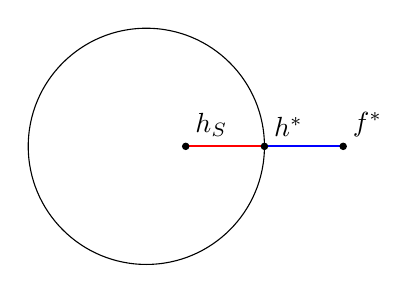
\begin{tikzpicture}[scale=.5]

    \draw (0,0) circle (3);
    
    \draw[thick,color=red](1,0) -- (3,0);
    \draw[thick,color=blue](3,0) -- (5,0);
    
    \draw[fill=black] (1,0) circle (.08);
    \node at (-2.75,2.75) {$\Hm$};
    \node[above right] at (1,0) {$h_S$};

    \draw[fill=black] (3,0) circle (.08);
    \node[above right] at (3,0) {$h^*$};

    \draw[fill=black] (5,0) circle (.08);
    \node[above right] at (5,0) {$f^*$};

\end{tikzpicture}
    \caption{Rappresentazione grafica della decomposizione \textit{bias-variance}}
\end{figure}